\subsection{Periodo Requirements and Technology Baseline}
\subsubsection{MPP1 - Schedule variance}

\begin{figure}[H]
	\centering
	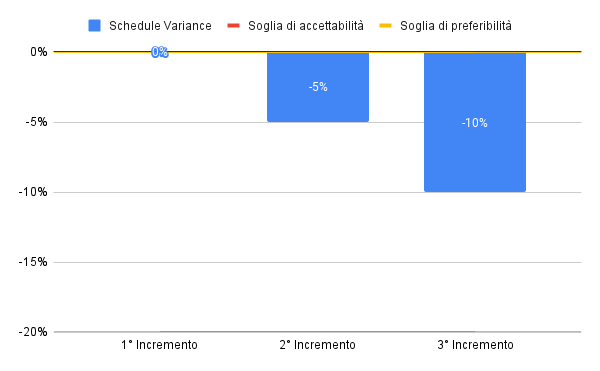
\includegraphics[scale = 0.6]{sezioni/Images/ScheduleVariance.png}
	\caption{MPP1 - Schedule variance}
\end{figure}

\subsubsection{MPP2 - Budget variance}

\begin{figure}[H]
	\centering
	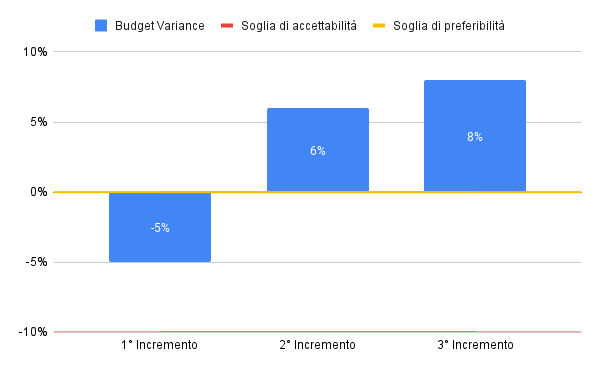
\includegraphics[scale = 0.6]{sezioni/Images/BudgetVariance.png}
	\caption{MPP2 - Budget variance}
\end{figure}

\subsubsection{MPP3 - SPICE capability}

\begin{figure}[H]
	\centering
	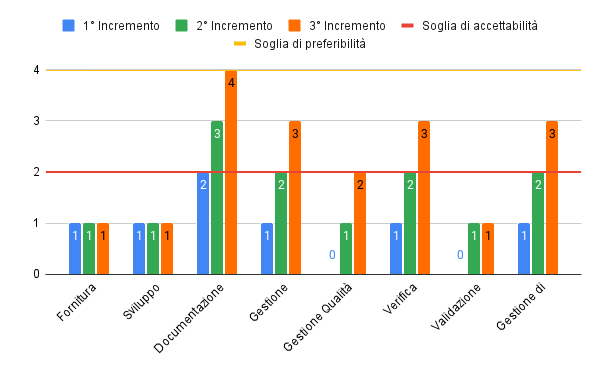
\includegraphics[scale = 0.6]{sezioni/Images/SPICECapability.png}
	\caption{MPP3 - SPICE capability}
\end{figure}

\subsubsection{MPP4 - Requirements Stability Index}

\begin{figure}[H]
	\centering
	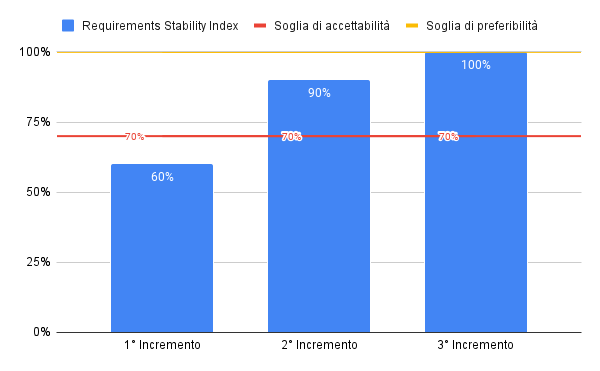
\includegraphics[scale = 0.6]{sezioni/Images/RequirementsStabilityIndex.png}
	\caption{MPP4 - Requirements Stability Index}
\end{figure}

\subsubsection{MPR1 - Indice di Gulpease}

\paragraph{Norme di progetto} \aCapo{}

\begin{figure}[H]
	\centering
	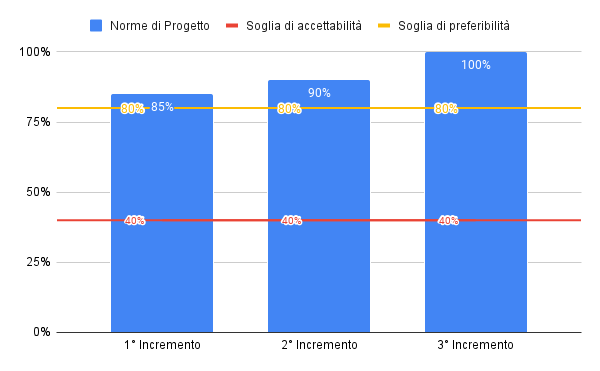
\includegraphics[scale = 0.6]{sezioni/Images/NdP.png}
	\caption{MPR1 - Indice di Gulpease delle norme di progetto}
\end{figure}

\paragraph{Piano di progetto} \textbf{•}

\begin{figure}[H]
	\centering
	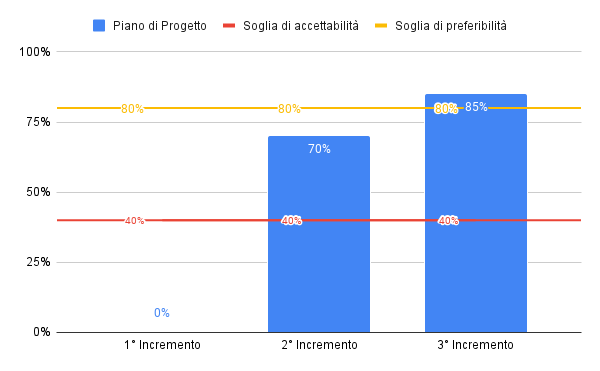
\includegraphics[scale = 0.6]{sezioni/Images/PdP.png}
	\caption{MPR1 - Indice di Gulpease del piano di progetto}
\end{figure}

\paragraph{Piano di qualifica} \aCapo{}

\begin{figure}[H]
	\centering
	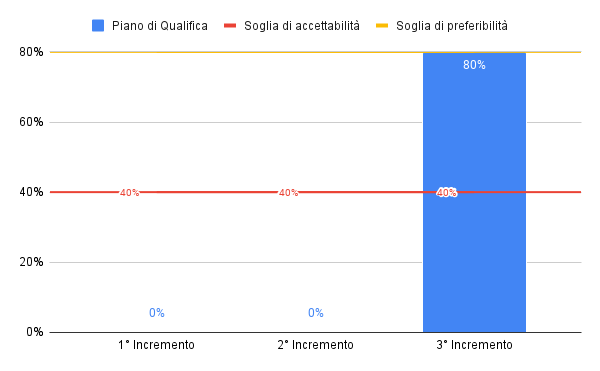
\includegraphics[scale = 0.6]{sezioni/Images/PdQ.png}
	\caption{MPR1 - Indice di Gulpease del piano di qualifica}
\end{figure}

\paragraph{Analisi dei requisiti} \aCapo{}

\begin{figure}[H]
	\centering
	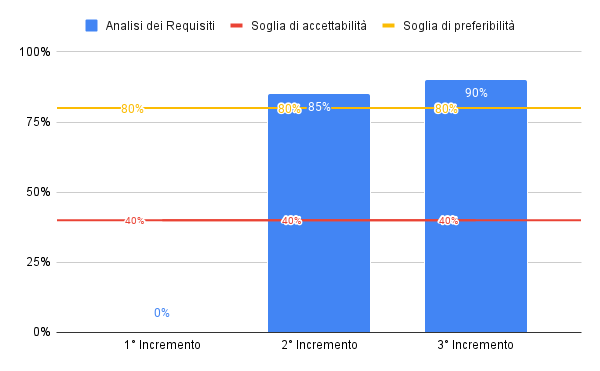
\includegraphics[scale = 0.6]{sezioni/Images/AdR.png}
	\caption{MPR1 - Indice di Gulpease dell'analisi dei requisiti}
\end{figure}

\paragraph{Glossario} \aCapo{}

\begin{figure}[H]
	\centering
	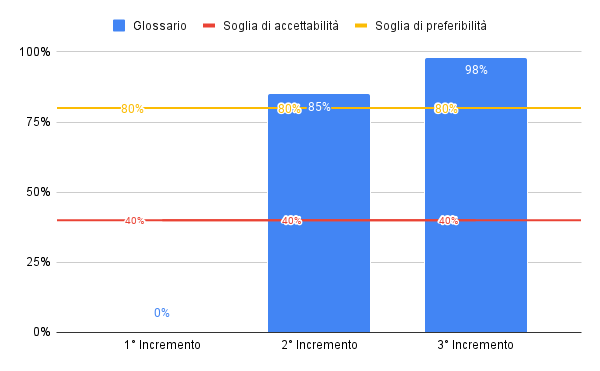
\includegraphics[scale = 0.6]{sezioni/Images/Glossario.png}
	\caption{MPR1 - Indice di Gulpease del glossario}
\end{figure}

\subsection{Product Baseline}
\subsubsection{MPP1 - Schedule variance}

\begin{figure}[H]
	\centering
	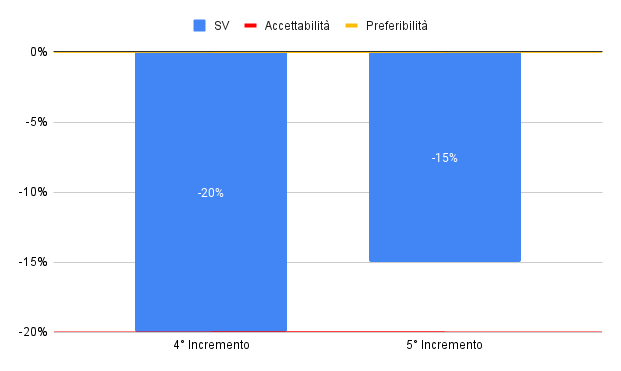
\includegraphics[scale = 0.6]{sezioni/Images/PB/SV.png}
	\caption{MPP1 - Schedule variance}
\end{figure}

\subsubsection{MPP2 - Budget variance}

\begin{figure}[H]
	\centering
	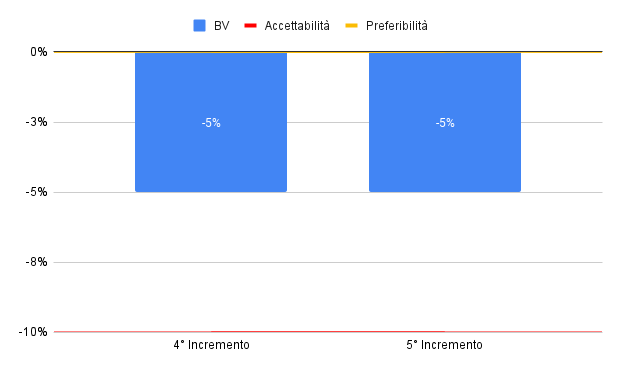
\includegraphics[scale = 0.6]{sezioni/Images/PB/BV.png}
	\caption{MPP2 - Budget variance}
\end{figure}

\subsubsection{MPP3 - SPICE capability}

\begin{figure}[H]
	\centering
	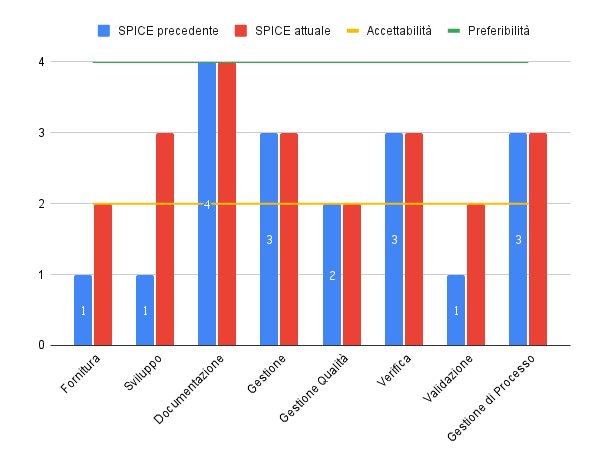
\includegraphics[scale = 0.6]{sezioni/Images/PB/SPICE.png}
	\caption{MPP3 - SPICE capability}
\end{figure}

\subsubsection{MPP4 - Requirements Stability Index}

\begin{figure}[H]
	\centering
	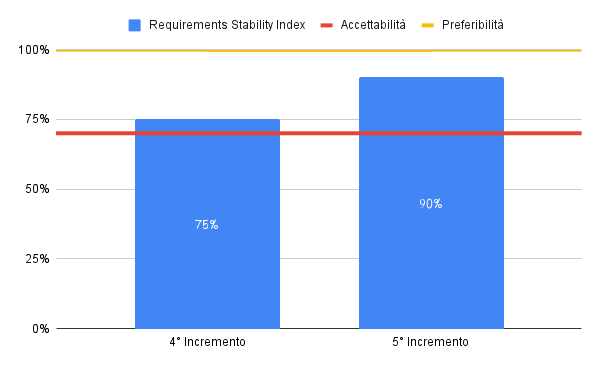
\includegraphics[scale = 0.6]{sezioni/Images/PB/RequirementsStabilityIndex.png}
	\caption{MPP4 - Requirements Stability Index}
\end{figure}

\subsubsection{MPR1 - Indice di Gulpease}

\begin{figure}[H]
	\centering
	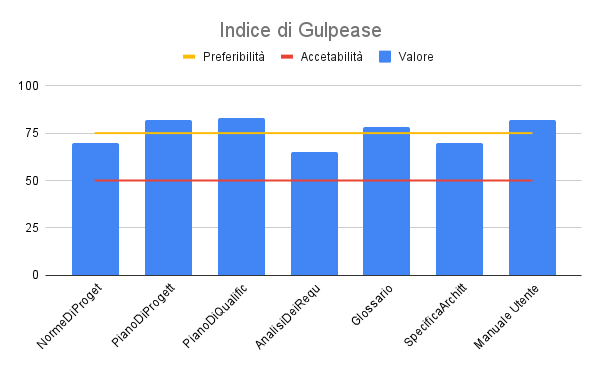
\includegraphics[scale = 0.6]{sezioni/Images/PB/GulpeaseGenerale.png}
	\caption{MPR1 - Indice di Gulpease dei documenti}
\end{figure}

\subsubsection{MPR3 - Code Coverage}

\begin{figure}[H]
	\centering
	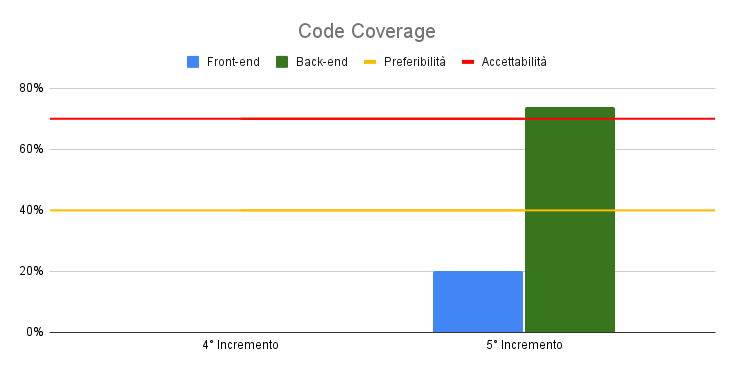
\includegraphics[scale = 0.6]{sezioni/Images/PB/CodeCoverage.png}
	\caption{MPR3 - Code Coverage}
\end{figure}

\subsubsection{MPR4 - Branch Coverage}

\begin{figure}[H]
	\centering
	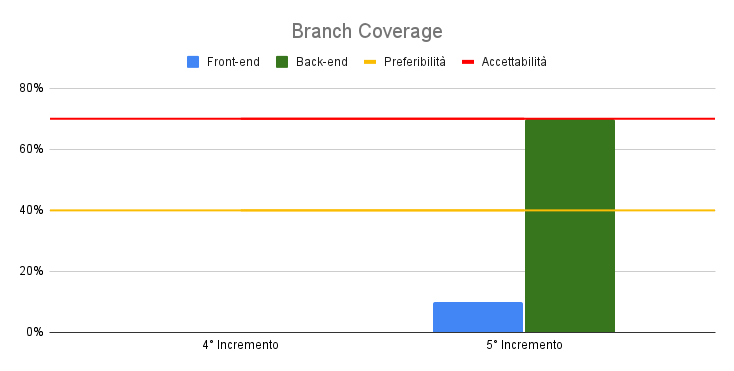
\includegraphics[scale = 0.6]{sezioni/Images/PB/BranchCoverage.png}
	\caption{MPR4 - Branch Coverage}
\end{figure}

\subsubsection{MPR6 - Profondità gerarchia}

\begin{figure}[H]
	\centering
	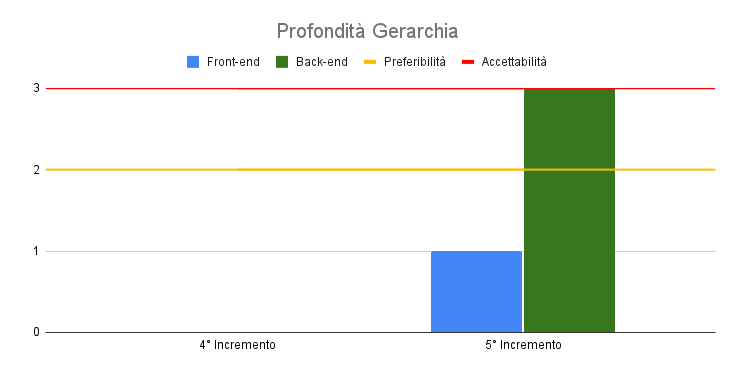
\includegraphics[scale = 0.6]{sezioni/Images/PB/Gerarchia.png}
	\caption{MPR6 - Profondità Gerarchie}
\end{figure}

\subsubsection{MPR7 - Numero parametri per metodo}

\begin{figure}[H]
	\centering
	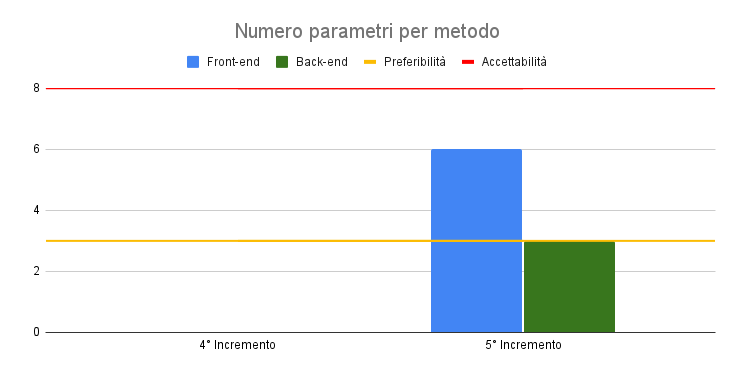
\includegraphics[scale = 0.6]{sezioni/Images/PB/ParamMetod.png}
	\caption{MPR7 - Numero parametri per metodo}
\end{figure}

\subsection{Collaudo}
\subsubsection{MPP1 - Schedule variance}
\begin{figure}[H]
	\centering
	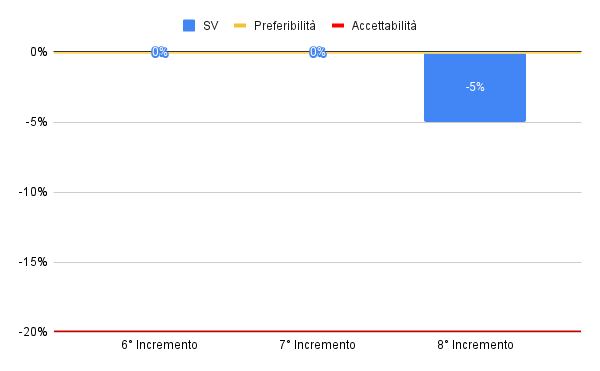
\includegraphics[scale = 0.6]{sezioni/Images/CA/SV.png}
	\caption{MPP1 - Schedule variance}
\end{figure}

\subsubsection{MPP2 - Budget variance}

\begin{figure}[H]
	\centering
	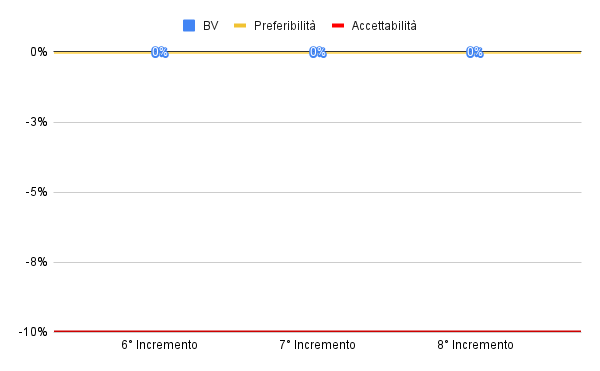
\includegraphics[scale = 0.6]{sezioni/Images/CA/BV.png}
	\caption{MPP2 - Budget variance}
\end{figure}

\subsubsection{MPP3 - SPICE capability}

\begin{figure}[H]
	\centering
	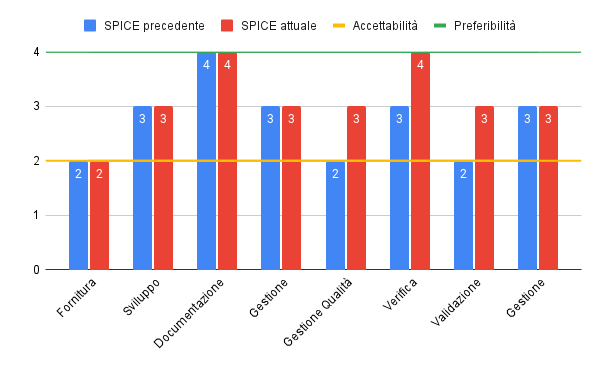
\includegraphics[scale = 0.6]{sezioni/Images/CA/SPICE.png}
	\caption{MPP3 - SPICE capability}
\end{figure}

\subsubsection{MPP4 - Requirements Stability Index}

\begin{figure}[H]
	\centering
	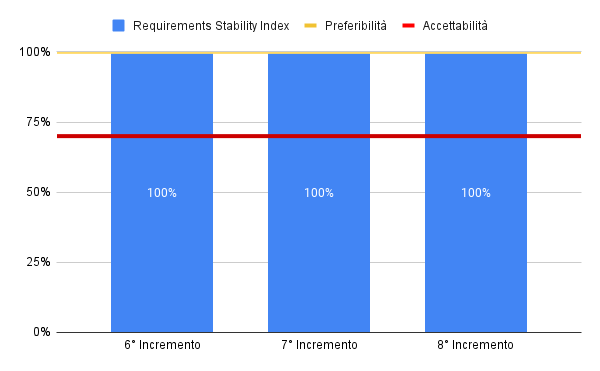
\includegraphics[scale = 0.6]{sezioni/Images/CA/RSI.png}
	\caption{MPP4 - Requirements Stability Index}
\end{figure}

\subsubsection{MPR1 - Indice di Gulpease}

\begin{figure}[H]
	\centering
	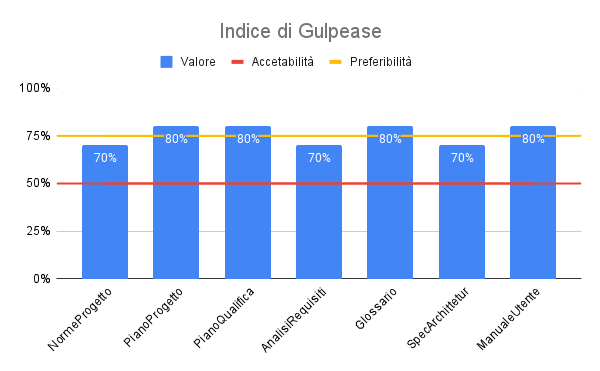
\includegraphics[scale = 0.6]{sezioni/Images/CA/GG.png}
	\caption{MPR1 - Indice di Gulpease dei documenti}
\end{figure}

\subsubsection{MPR3 - Code Coverage}

\begin{figure}[H]
	\centering
	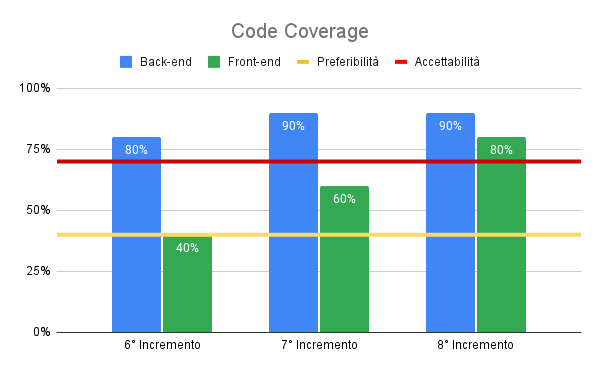
\includegraphics[scale = 0.6]{sezioni/Images/CA/CC.png}
	\caption{MPR3 - Code Coverage}
\end{figure}

\subsubsection{MPR4 - Branch Coverage}

\begin{figure}[H]
	\centering
	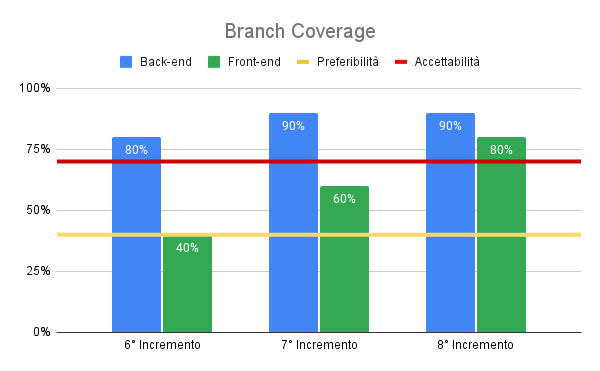
\includegraphics[scale = 0.6]{sezioni/Images/CA/BC.png}
	\caption{MPR4 - Branch Coverage}
\end{figure}

\subsubsection{MPR6 - Profondità gerarchia}

\begin{figure}[H]
	\centering
	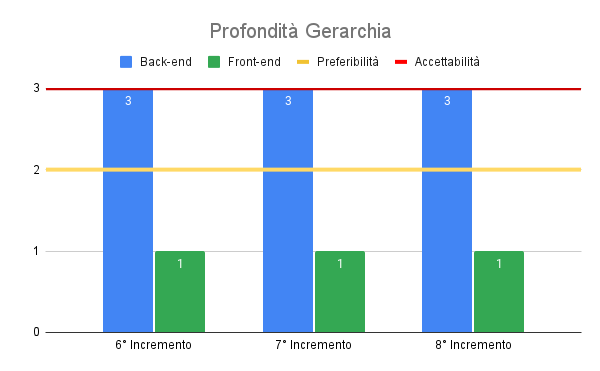
\includegraphics[scale = 0.6]{sezioni/Images/CA/PG.png}
	\caption{MPR6 - Profondità Gerarchie}
\end{figure}

\subsubsection{MPR7 - Numero parametri per metodo}

\begin{figure}[H]
	\centering
	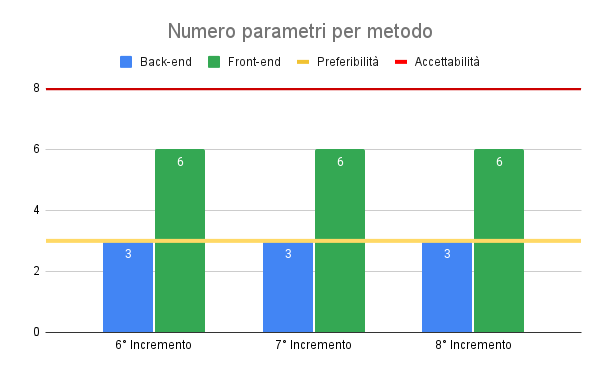
\includegraphics[scale = 0.6]{sezioni/Images/CA/PM.png}
	\caption{MPR7 - Numero parametri per metodo}
\end{figure}